\documentclass{article}

% if you need to pass options to natbib, use, e.g.:
%     \PassOptionsToPackage{numbers, compress}{natbib}
% before loading neurips_2018

% ready for submission
% \usepackage{neurips_2018}

% to compile a preprint version, e.g., for submission to arXiv, add add the
% [preprint] option:
\usepackage[preprint]{neurips_2018}

% to compile a camera-ready version, add the [final] option, e.g.:
% \usepackage[final]{neurips_2018}

% to avoid loading the natbib package, add option nonatbib:
%     \usepackage[nonatbib]{neurips_2018}

\usepackage[utf8]{inputenc} % allow utf-8 input
\usepackage[T1]{fontenc}    % use 8-bit T1 fonts
\usepackage{hyperref}       % hyperlinks
\usepackage{url}            % simple URL typesetting
\usepackage{booktabs}       % professional-quality tables
\usepackage{amsfonts}       % blackboard math symbols
\usepackage{nicefrac}       % compact symbols for 1/2, etc.
\usepackage{microtype}      % microtypography
\usepackage{graphicx}

\title{Initial Report: Alberta Election Data 2015-2019}

\author{%
  Sam Mikes \\
  \texttt{smikes@apple.com} \\
  % examples of more authors
  % \And
  % Coauthor \\
  % Affiliation \\
  % Address \\
  % \texttt{email} \\
}
\begin{document}
\maketitle

\begin{abstract}
  Election data for Alberta for 2015-2019 is collected
  from government open data sources and analyzed with unsupervised
  learning. Geographic correlation to 2016 Canada census.
\end{abstract}

\section{Data Sources}

Results are available for municipal, provincial, and federal elections.
The initial analysis will use only the 2015 Provincial Election results to validate methods. 

\subsection{Provincial}

2015 Election results and geography

\url{https://open.alberta.ca/opendata/2015-general-election-results}

\subsection{2016 Census and Geography}

Canada Census data for Alberta is available by geography, organized by 'Census Divisions' (CDs: 20), 'Census Subdivisions' (CSDs: 425), 'Dissemination Areas' (DAs: 5803).  Initially we hoped to use 'Dissemination Blocks', which are even smaller than DAs.  Becuase Dissemination Blocks may be too small to maintain the privacy of census respondents, we chose to use only DA and larger-sized units.

\section{Design}

In the 2015 election, there were 87 electoral districts (EDs). For each district, results are reported by 'Poll', where a Poll may be a geographic subset of the district, or a virtual/logical entity such as 'Advance Votes', 'Mail-in Votes', 'Mobile Poll 1'.

Initial analysis attempted to connect results by poll to census data at dissemination areas.  This problem (2247x3 features ; 5803 DAs ; 6269 Polls) was difficult to approach.  Specifically, the multiple overlaps between census DAs and polls (see figure 1) were difficult to model.

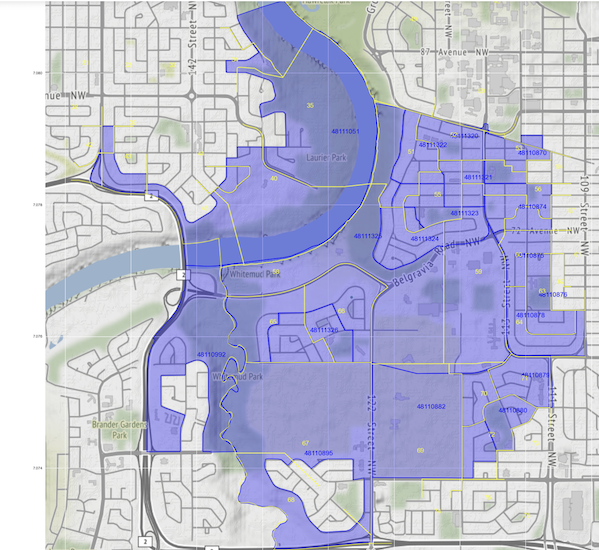
\includegraphics[scale=0.4]{figure1-da-poll-overlap-small.png}

To validate the approach, we followed the suggestion of Gu (personal communication) to first examine the 87 electoral districts in relation to the CSDs.  This problem proved to be easily approached with PCA and linear regression, which suggests that dimension reduction should be applied to the larger problem (polls <-> DAs).

\section{Data Conditioning}

\subsection{2015 Electoral Results}

Alberta's 2015 provincial election results are reported in a human-friendly Excel format, with column headers varying by the presence of particular party candidates in any given district.  A custom python script was written to produce a consistent, flattened summary (data/interim/2015-pge.csv).

For initial analysis, this was further reduced to a sum of votes cast by electoral districts for the three political parties of interest in 2015: New Democratic Party, Progressive Conservative Party, Wild Rose Party.  Both the number of registered votes and the number of valid votes were retained for reference.  (data/interim/votes-riding-2015.csv.gz)

\subsection{2016 Census}

The 2016 census reports direct variables (from immediate answers to questions); derived variables (such as median or average income); and coded variables.  To simplify the initial analysis, the 2247 reported variables were reduced.

First, the distribution of variables across 'level' was evaluated.  Level is indicated by the indentation in the `census-value-structure.txt` file supplied by Statistics Canada.  The distribution of features by level is documented in table 1.

\begin{table}[h]
\begin{tabular}{ll}
level 0 & 108  \\
level 1 & 440  \\
level 2 & 936  \\
level 3 & 1241 \\
level 4 & 1457 \\
level 5 & 1855 \\
level 6 & 2133 \\
level 7 & 2247
\end{tabular}
\caption{Canada Census 2016 Variable Levels}
\label{tab:table1}
\end{table}

We chose to cut at level 2, which meant that 936 variables were retained for further analysis.  Because each variable may be reported as Total, Male, Female when appropriate, this is still >2000 features.

Variables with 'Average', 'Median' or 'Total' in the name were dropped, as these are presumptively derived variables.  Variables which were always 0 in the Alberta CSD subset were also removed at this point.  The resulting data was unstacked to form a single matrix (425 rows x 1232 columns) containing the census features at levels 0, 1, and 2 that were not obviously dependent on other features.

\subsection{Geographic Correlation}

Geographic correlation was determined by evaluating whether there was overlap between two geometries; if there was overlap, a binary feature (BIN-OVERLAP) was set for that combination of ED and CSD.  Overlap was calculated in the commonly-used EPSG:3857 coordinate reference, because of the easy availability of free maps for that CRS.  Overall, there were 756 overlaps, and the median overlap of 0.98 indicated that for half the census subdivisions, the subdivision lay almost completely within one ED.  Similarly, the 25th percentile overlap (0.0097) indicated that 1/4 of overlaps were nearly insignificant.

After correlation, the census variables were summed by ED, producing a raw data table of 87 EDs x 1232 census features.

\subsection{Target Data}

To investigate PCA, we chose two endpoints of interest: the proportion of votes cast in 2015 that went to the NDP (socialist) party on the one hand, and the proportion of votes that went to one of the two conservative parties (Wild Rose and PC).  These very nearly sum to 1, so they cannot be considered as independent; more work should be done to check the validity of the PCA.

\section{Analysis}

Using Scikit-Learn, PCA followed by linear regression was applied to the data. The maximum possible rank is 87; accordingly, we evaluated the $r^2$ score for $n_{components}$ between 1 and 60.  The initial result is that score rises rapidly at first, and flattens off at about 15 components.  See figure 2.

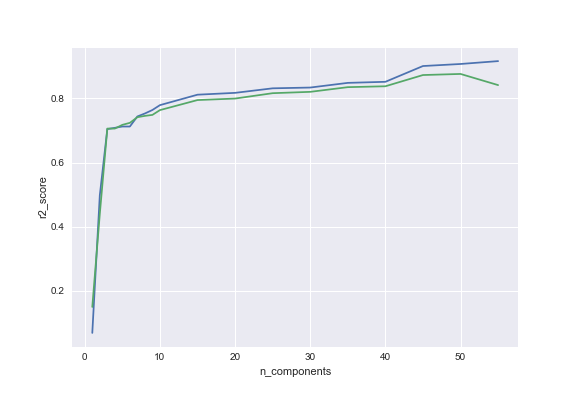
\includegraphics[scale=0.4]{figure2-pca.png}

\subsection{Future Work}

The next step is to standardize the dimension-reducing PCA matrix and use it to reduce the DA-level census data to a more tractable size.  Then we can investigate whether any meaningful difference is made by weighting the DAs equally (as we have done so far), or in proportion to the overlap area between the DA and the Poll to the total area of the DA.

Separately, an investigation into which census variables are most relevant to the computed principal components should be done, to produce a model with more meaningful independent variables.

Other endpoints such as the fraction of votes for each Conservative party, or voter turnout should also be evaluated in order to confirm that the resolved principal components robustly predict more than one result of interest.

\section{Conclusion}

When using census data to predict results, one must first focus on an appropriate dimension reduction.

\medskip

\small


\end{document}
